\chapter{The Indian Court System}
\label{ch:india}

\begin{quote}\itshape
Law is the method, the manner in which our mind grasps a series of phenomena; it is all in the mind.
\par\hfill\normalfont Swami Vivekananda, \emph{Karma Yoga}
\end{quote}

\section{A common law system at scale}

India inherited the common law from British rule and has developed it into one of the world's most important legal systems. Its Supreme Court is among the most powerful constitutional courts anywhere; its High Courts have broad original and writ jurisdiction; its district and subordinate courts handle tens of millions of matters. It also carries the largest judicial backlog in the world. In July 2026 the Law Minister told Parliament, citing the National Judicial Data Grid, that more than $4.99$ crore cases were pending in subordinate courts, about $64.67$ lakh in the High Courts and about ninety three thousand in the Supreme Court (the last figure as on 28 July 2026), some $5.6$ crore, or fifty six million, in all. Parliamentary replies the same month put the High Court cases pending for more than thirty years at over seventy thousand (71,204 as on 24 July, 80,634 as on 28 July).\index{India!pendency}

This chapter describes the structure of the Indian courts, the evidence law that governs them, the causes and consequences of delay, and the use of data and technology to manage it. Its main argument is that delay is a decision problem: a court system with fixed capacity must decide which cases to hear, in what order, and how much time to give each, and Bayesian decision theory gives a principled way to make those choices.

\section{Vivekananda on law}

Swami Vivekananda, lecturing in America and England in the 1890s, gave an account of law that a Bayesian will find congenial. In his lectures on Karma Yoga he defined law as the tendency of a series to repeat itself, and argued that our idea of law arises from association: when phenomena recur in a regular order, the mind forms the expectation that they will recur, and that expectation is what we call a law. He connected this with the notion that the Nyaya school of Indian logic called \emph{vyapti}, the invariable concomitance on which inference rests \citep{vivekananda1896}. Law, he concluded, is the method, the manner in which our mind grasps a series of phenomena.\index{Vivekananda, Swami}\index{vyapti}

Vivekananda was speaking of natural and spiritual law, not of statutes. But his account describes the common law closely. A rule of the common law is the regularity a court perceives in a series of decided cases; precedent is the expectation that like cases will be decided alike; and a judge who distinguishes a precedent is recognising that the series does not extend to the case before her. In the hierarchical model of Chapter~\ref{ch:commoncivil}, the rule is the posterior summary of many decisions, the unity found in their variety. The Nyaya theory of inference, which required that the concomitance on which an inference rests be established by repeated observation and checked against counterexamples, is a theory of induction from cases of the kind the common law practises. India's courts, which apply a common law inherited from England in a country whose own traditions of logic and law are far older, are a natural place to notice the connection.

\section{Structure}

\subsection{The courts}

The Supreme Court, established by Article 124 of the Constitution, hears appeals from the High Courts and petitions for the enforcement of fundamental rights under Article 32. Under Article 136 it may grant special leave to appeal from any judgment of any court or tribunal, a discretionary jurisdiction that brings a large number of petitions to the Court. Under Article 142 it may pass any decree or order necessary for doing complete justice in any cause before it. The High Courts, twenty five in number, have supervisory jurisdiction under Article 227 and writ jurisdiction under Article 226 that is wider than the Supreme Court's, since it extends to the enforcement of legal rights generally. Below them, district courts and subordinate courts, civil and criminal, handle the great majority of cases.\index{Supreme Court of India}

\subsection{Public interest litigation}

From the late 1970s the Supreme Court relaxed rules of standing and procedure to allow public interest litigation. Letters to judges were treated as petitions; the Court appointed commissions to gather facts; and it issued continuing orders supervising government action. In \emph{Hussainara Khatoon v Home Secretary, State of Bihar}, a 1979 case brought on the basis of newspaper reports, the Court held that the right to a speedy trial is part of the right to life and personal liberty under Article 21 and ordered the release of undertrial prisoners who had been detained for longer than the maximum sentence for the offences charged \citep{hussainara1979}. Public interest litigation gave the Court a role in governance unmatched by most courts, and it also added to the Court's load.\index{public interest litigation}

\subsection{Lok Adalats}

The Legal Services Authorities Act 1987 gave statutory status to Lok Adalats, people's courts, which resolve disputes by conciliation and compromise. An award of a Lok Adalat is deemed a decree of a civil court and is final, with no appeal. National Lok Adalats held on single days across the country dispose of large numbers of matters, both pending cases and disputes at the pre litigation stage, especially in motor accident claims, cheque dishonour, family disputes and bank recovery. They are a parallel disposal channel that relies on the parties' willingness to settle.\index{Lok Adalat}

\section{The law of evidence}

\subsection{Stephen's definition of proof}

The Indian Evidence Act 1872 was drafted by James Fitzjames Stephen, who sought to codify the English law of evidence in a form that Indian judges, many of them not trained in English law, could apply. Section 3 defined proof in terms that a decision theorist would recognise:
\begin{quote}
A fact is said to be proved when, after considering the matters before it, the Court either believes it to exist, or considers its existence so probable that a prudent man ought, under the circumstances of the particular case, to act upon the supposition that it exists.
\end{quote}
The definition has two parts. The first is belief. The second is probability combined with action: the fact is proved when its probability is high enough that a prudent person ought to act on it under the circumstances. That is the decision theoretic standard of Chapter~\ref{ch:standards}: a posterior threshold that depends on the consequences of acting, which differ from case to case. Stephen wrote, nearly a century before Kaplan, a definition of proof that ties the threshold to the stakes.\index{Indian Evidence Act}\index{Stephen, James Fitzjames}

The Indian courts have read the definition as permitting different standards in criminal and civil cases, with proof beyond reasonable doubt required in the former, and as emphasising the prudent man's judgment in the circumstances. In 2023 Parliament replaced the Indian Penal Code, the Code of Criminal Procedure and the Evidence Act with three new statutes, the Bharatiya Nyaya Sanhita, the Bharatiya Nagarik Suraksha Sanhita and the Bharatiya Sakshya Adhiniyam, which came into force in July 2024. The new evidence statute retains Stephen's definitions of proved, disproved and not proved, while modernising provisions on electronic records.

\subsection{Presumptions}

Stephen's Act also codified presumptions, including the court's power under section 114 to presume the existence of any fact it thinks likely to have happened, having regard to the common course of natural events, human conduct and public and private business. The illustrations to the section are a catalogue of prior probabilities: that a man in possession of stolen goods soon after the theft is either the thief or has received the goods knowing them to be stolen, unless he can account for his possession; that an accomplice is unworthy of credit unless corroborated in material particulars; that a bill of exchange was accepted for good consideration. Each presumption is a default probability given the basic fact, which serves as the prior for any rebutting evidence. The Bayesian framework explains why presumptions are useful: they economise on proof by fixing the prior where experience supports it, and they place the burden of producing contrary evidence on the party best placed to produce it.

\section{Delay}

\subsection{Causes}

Many causes of delay have been identified: too few judges relative to population and caseload, vacancies in sanctioned posts, frequent adjournments, the government's role as the largest litigant and its tendency to appeal adverse decisions, procedural complexity, the volume of minor cases such as cheque dishonour prosecutions, and inadequate infrastructure. The Law Commission recommended in its 1987 report a ratio of fifty judges per million population; the actual ratio has remained a fraction of that.\index{judge population ratio}

\subsection{Consequences}

Delay imposes direct costs on litigants and indirect costs on the economy. For criminal defendants held in custody awaiting trial, delay is punishment without conviction. Undertrial prisoners make up a large majority of India's prison population, and many are poor and unable to meet bail conditions. For commercial parties, delay reduces the value of contracts, as Chapter~\ref{ch:africa} described for African courts, and encourages reliance on relationships rather than law. For the legitimacy of the courts, delay undermines the belief that rights can be enforced.

\section{A queueing model}

A court system is a queue. Cases arrive, wait, are served and leave. Let $B_t$ be the number of pending cases at the start of year $t$, $A_t$ the number filed during the year and $D_t$ the number disposed of. Then
\begin{equation}
B_{t+1} = B_t + A_t - D_t .
\end{equation}
If arrivals exceed disposals, the backlog grows without bound. If disposals exceed arrivals, it shrinks. Little's law, a basic result of queueing theory, says that in a steady state (arrivals equal to disposals, which only roughly describes India) the average time a case spends in the system equals the average number pending divided by the throughput:
\begin{equation}
\bar W = \frac{\bar B}{\bar D}.
\end{equation}
With a backlog of about $5.6$ crore and annual disposals of the order of two to two and a half crore, the average time in the system is two to three years, and the distribution is highly skewed, with some cases pending for decades.\index{queueing model}\index{Little's law}

Figure~\ref{fig:indiabacklog} shows stylised backlog paths under different disposal rates, holding arrivals fixed. The point is the sensitivity: a small excess of arrivals over disposals produces steady growth, and even a disposal rate a sixth above arrivals takes fourteen years to clear the backlog. Raising disposals requires more judges, fewer adjournments, simpler procedures or diversion of cases to other channels such as Lok Adalats.

\begin{figure}[t]
\centering
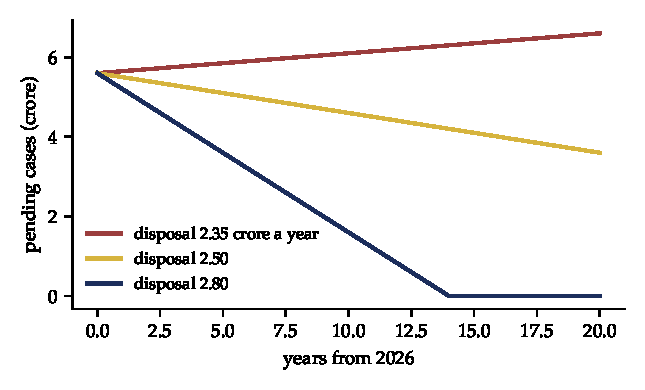
\includegraphics[width=\linewidth]{fig_india_backlog}
\caption{Stylised paths of the total pending caseload under three annual disposal rates, starting from $5.6$ crore with arrivals fixed at $2.4$ crore a year. Illustrative values, not forecasts.}
\label{fig:indiabacklog}
\end{figure}

\section{Bayesian triage}

\subsection{Which cases first}

If a court cannot hear every case promptly, it must decide which to hear first. The default in most courts is first come, first served, modified by statutory priorities and judicial discretion. Queueing theory offers a better rule when cases differ in the cost of delay and in the time needed to decide them. The $c\mu$ rule says that to minimise the total cost of waiting, when delay costs are linear in time and there is a single server, a server should give priority to the class of jobs with the highest product of the cost of delay per unit time, $c$, and the service rate, $\mu$, the reciprocal of the expected service time. Short cases with high costs of delay go first; long cases with low costs of delay wait.\index{c mu rule}

In a court, the cost of delay depends on the case: an undertrial prisoner's detention, a family without access to its land, a business with funds frozen. The service time depends on the complexity of the case and the likelihood of adjournment. Neither is known exactly at filing. A Bayesian triage system would estimate both from the case's features, using a hierarchical model trained on past cases, and would update the estimates as the case progresses. The priority index for case $j$ is then
\begin{equation}
\pi_j = \frac{\E[c_j \given \text{data}]}{\E[1/\mu_j \given \text{data}]},
\end{equation}
the expected cost of delay divided by the expected service time, or, taking account of uncertainty, a quantity such as the Gittins index, which values a case by the best long-run rate of return from working on it and so rewards learning about uncertain cases.

\subsection{Value of information}

Some cases can be resolved quickly once a single question is answered: whether a cheque was presented within time, whether a notice was served, whether the parties are willing to compromise. The value of information calculation of Chapter~\ref{ch:standards} identifies cases where a small investment of judicial time would likely produce a disposal. A triage system that screens cases for such questions, perhaps referring them to a short hearing or to a Lok Adalat, could raise disposals without new judges.

\subsection{Adjournments}

Adjournments are a major cause of delay. Each adjournment is a decision by the court to postpone, often at a party's request. A model of adjournments would estimate the probability that a hearing results in adjournment as a function of the case, the stage, the parties and the court, and would identify where adjournments are concentrated. Reforms such as costs on parties who seek adjournments, limits on their number, or case management conferences that fix timetables, can then be targeted. The data to estimate such models exist in the National Judicial Data Grid.

\section{Data and technology}

\subsection{The National Judicial Data Grid}

The eCourts project, a mission mode programme of the government and the judiciary, has computerised the district courts and created the National Judicial Data Grid, a public platform that reports pending and disposed cases by court, case type and age, updated continuously. The Grid makes Indian court data among the most accessible in the world. It allows researchers, journalists and the courts themselves to see where backlogs are concentrated and how they change. It is the foundation for any data driven approach to court management.\index{National Judicial Data Grid}

\subsection{Artificial intelligence}

The Supreme Court has introduced artificial intelligence tools for translation of judgments into Indian languages and for assisting judges with research. The use of such tools raises the questions to which Chapter~\ref{ch:lindleyai} returns: accuracy, bias, transparency and the proper division of labour between the machine and the judge. For a court system under the load India's carries, the potential benefits of automation in routine tasks, such as scheduling, translation, document review and the identification of similar cases, are large. The risks are greatest where machines would make or shape decisions on liberty or rights, and there the Bayesian requirements of calibration and explicit uncertainty are most important.

\section{Bail as expected utility}

The bail decision illustrates the use of probability in an Indian court under load. A magistrate deciding whether to release an accused before trial must weigh the risk that the accused will abscond, tamper with evidence or commit further offences against the cost of detention to the accused, who is presumed innocent and may wait years for trial. Let $r$ be the probability of a harmful event if released, $H$ the harm, and $C$ the cost of detention (the loss called $D$ in Chapter~\ref{ch:decisions}, renamed here because $D_t$ denotes disposals) over the expected time to trial $T$. Release is the better decision if
\begin{equation}
r\,H < (1-r)\,C(T),
\end{equation}
as in Chapter~\ref{ch:decisions}, and $C(T)$ grows with $T$. In a system where trials take years, $C(T)$ is large, and release should be the norm for all but high risk accused. In \emph{State of Rajasthan v Balchand} (1977) the Supreme Court put the basic rule as \textquotedblleft bail, not jail\textquotedblright, and it has repeated since that bail is the rule and jail the exception. The decision theoretic analysis supports that principle, and shows that it becomes stronger as delay increases. Risk assessment tools that estimate $r$ could help magistrates, but they must be calibrated on Indian data and checked for bias, as Chapter~\ref{ch:lindleyai} explains.

\section{Lessons}

India shows that the common law's reliance on courts to resolve disputes and make law requires courts with capacity to match demand. When capacity falls short, delay becomes the dominant feature of the system, and the theoretical virtues of adversarial procedure and precedent are swamped. Stephen's Evidence Act, with its decision theoretic definition of proof, shows that decision theoretic ideas were built into Indian evidence law from 1872. The National Judicial Data Grid shows what transparency about the state of the courts can achieve. The next step is to use those data for decisions: which cases to hear, which to divert, how to schedule, and when to release. Each is a decision under uncertainty, and each can be improved by explicit probabilities and costs.

\section*{Notes and Questions}
\addcontentsline{toc}{section}{Notes and Questions}
\begin{enumerate}[label=\arabic*.]
\item Read section 3 of the Indian Evidence Act and section 2 of the Bharatiya Sakshya Adhiniyam. Express the definition of proved as a decision rule. What role does the phrase under the circumstances of the particular case play?
\item Using Little's law, compute the average time to disposal for a court with a backlog of two hundred thousand cases and annual disposals of eighty thousand. What disposal rate would halve it?
\item A court has two classes of case: bail applications with an expected hearing time of ten minutes and a cost of delay of one unit per day, and civil suits with an expected hearing time of three hours and a cost of delay of two units per day. Apply the $c\mu$ rule.
\item Section 114 of the Evidence Act allows courts to presume facts likely to have happened. Choose three illustrations to the section and state the prior probability each implicitly assumes.
\item Design a Bayesian model of adjournments using data of the kind available in the National Judicial Data Grid. What variables would you include, and how would you use the model to target reform?
\item Using the bail inequality, find the maximum risk of absconding at which release is optimal if the harm from absconding is ten units, the cost of detention is one unit per month and the expected time to trial is two years.
\end{enumerate}

\section*{Further reading}
The National Judicial Data Grid is the primary source for data. Stephen's own \emph{Digest of the Law of Evidence} explains his approach. On public interest litigation, \emph{Hussainara Khatoon} \citep{hussainara1979}.
